As this project is purely an investigation into whether a more modern solution for transferring files can be produced, these prototypes will only focus on the minimum possible required to have functionality. This allows for each prototype to improve on the most important features. These are listed below:

\begin{itemize}
	\item Error correction
	\item Sending files from client to server
	\item Adjustable settings, for testing
	\item Only support a single client connection
\end{itemize}

To test the prototypes, the previous methodology of testing will be used. This is documented in Appendix~\ref{sec:testing-environment}. On the virtualised network, these prototypes will use the maximum available MTU size which is 65,000 bytes which matches the previous tests.

Below are links for the prototype source code:

\begin{itemize}
    \item Prototype One: \url{https://github.com/enchant97/file-sync-protocol/tree/main/prototypes/proto-1}
    \item Prototype Two: \url{https://github.com/enchant97/file-sync-protocol/tree/main/prototypes/proto-2b}
    \item Prototype Three: \url{https://github.com/enchant97/file-sync-protocol/tree/main/prototypes/proto-3}
\end{itemize}

\newpage
\section{Prototype One}
\subsection*{Solution Design}
The first prototype will take inspiration from FTP streaming for file data transfer. Using UDP with this should reduce the total latency for a transfer; since all file data packets can be sent with no interruption for waiting for acknowledgments.

This prototype will use the binary protobuf format for structuring the packet data. This will reduce the amount of required overhead needed for storing structured data. Binary is suited for this prototype since it does not need to be easily human readable since only the software will be directly interacting with the data.

\subsubsection*{Packet Structure}
The packets structure will be split into several fields, using flexible offsets meaning the packet size is dynamic. Having a dynamic packet size should reduce the amount of wasted space, leaving more available space for the actual file data.

A packet will feature two protobuf fields one for the header which will describe what the packet is, and the second will include any extra metadata relevant to a request/response. The packets fields are illustrated in Table~\ref{tab:p1d-packet-fields}.

\begin{table}[h!]
    \caption{Prototype One Packet Fields}
    \label{tab:p1d-packet-fields}
    \centering
    \begin{tabular}{ l l l }
        \hline
        \textbf{Num} & \textbf{Name}   & \textbf{Data-Type} \\
        \hline
        001          & Type            & uint8              \\
        \hline
        002          & Header Length   & uint64             \\
        \hline
        003          & Header          & protobuf           \\
        \hline
        004          & Metadata Length & uint64             \\
        \hline
        005          & Metadata        & protobuf           \\
        \hline
        006          & Payload Length  & uint64             \\
        \hline
        007          & Payload         & binary             \\
        \hline
    \end{tabular}
\end{table}

The first field will take up exactly 1 byte, this field will be used to set the type of the packet. This will determine what protobuf encoded header structure will be. Using 1 byte will allow for 255 possible message types. Since these prototypes will not be a fully implemented solution only a few types will be implemented, which are shown in Table~\ref{tab:p1d-packet-types}.

\begin{table}[h!]
    \caption{Prototype One Packet Types}
    \label{tab:p1d-packet-types}
    \centering
    \begin{tabular}{ l l l }
        \hline
        \textbf{Prefix} & \textbf{Value} & \textbf{Note}                \\
        \hline
        SYN             & 1              & Perform connection handshake \\
        \hline
        ACK             & 2              & Acknowledge request          \\
        \hline
        REQ             & 3              & Request to send/receive      \\
        \hline
        PSH             & 4              & Send payload data            \\
        \hline
        FIN             & 254            & End connection               \\
        \hline
    \end{tabular}
\end{table}

The next field will take up 8 bytes, this will be big-endian ordered number which will say how many bytes of data to expect after for the header (an offset value).

After header length the actual header will follow, if there is no header the next field will immediately follow.

The 4th field will be the metadata length which is the same as the header length, however specifies the length of the metadata field.

The metadata field is the same as the header.

An example of a SYN packet in both a structured view and a hex representation of the binary data is shown in Listing~\ref{lst:p1d-example-structure} and Listing~\ref{lst:p1d-example-binary}.

\begin{minipage}{\textwidth}
    \begin{lstlisting}[caption={Prototype One Example Packet Structure},label=lst:p1d-example-structure]
|-------------------|
| 1                 | <- Packet Type
| 5                 | <- Header Length
| {id: 1, mtu: 470} | <- Protobuf Header (JSON representation)
| 0                 | <- No Metadata
| 0                 | <- No Payload
|-------------------|
\end{lstlisting}

    \begin{lstlisting}[caption={Prototype One Example Packet Binary},label=lst:p1d-example-binary]
 1 0 0 0 0 0 0 0 5 8 1 16 214 3 0 0 0 0 0 0 0 0 0 0 0 0 0 0 0 0
 ^ ^^^^^^^^^^^^^^^ ^^^^^^^^^^^^ ^^^^^^^^^^^^^^^ ^^^^^^^^^^^^^^^
 |        |             |              |               |
Type    Header        Header        Metadata        Payload
        Length                       Length         Length
\end{lstlisting}
\end{minipage}

\subsubsection*{Operation}
For a client to first connect to the server a simple handshake will occur. This has been based on the rsync protocol handshake which only requires one exchange at the start. The client will first send a packet type called "SYN" which includes the clients max receiving MTU size, this allows for the message size to be adjusted depending on the network structure. After the server has received it will acknowledge the handshake and send back it's own "SYN" packet, which will contain it's maximum supported receiving MTU and a generated client ID. This client ID will be stored at the server until the client disconnects, this will allow for a connection to remain available without the client needing to renegotiate. Because this ID will be used to determine which client is which, each message sent by the client will need this ID attached. Every message from the client following "SYN", must also increment a request ID field, which will allow error checking functionality.

Since UDP is used error handling for missing and out-of-order packets is needed and for the server to know when the client has received the response from the server. This is already a implemented feature in TCP, so this prototype will be based off how TCP works. Each request message sent from the client will expect a "ACK" packet which will contain the request ID in the header, so the client can handle out-of-order and missing messages. There will a timeout duration for waiting for a "ACK", after the timeout the original message will be sent again. This will repeat until a "ACK" is received.

After a handshake, the client is free to send a request which in this prototype; will either be a request to send a file or ending the connection.

To request to send a file; a packet type of "REQ" is sent with the destination file path and file size in the packets metadata field, including the size allows the server to decide whether there is enough space to receive the file and reserve it. The server will reply with an "ACK" and the client will send the file data in a streaming fashion, each packet will be a "PSH" type containing the chunk ID and the request ID. A chunk ID is needed to reconstruct the received data at the server side so it is in the correct order, this ID is simply a incrementing number. The "PSH" packets will not have "ACK" responses from the server, instead validation will happen after the transfer. This has been designed to reduce the latency during a transfer since most networks have little to no packet loss.

Once a transfer is finished the client will send a "REQ" packet containing the last chunk ID. The client will then either receive a "ACK" from the server if no chunks are missing, or a "REQ" packet containing the missing chunks; causing the client to send "PSH" packets containing the missing chunks. This will repeat until a "ACK" is received.

To end a connection, the client will send a "FIN" packet, this will include just the client ID. The server will recognise the request to end and clear the client ID and "ACK" the request.

A sequence diagram example of a complete transfer is shown in Figure~\ref{fig:p1-sequence}.

\begin{figure}[h!]
    \centering
    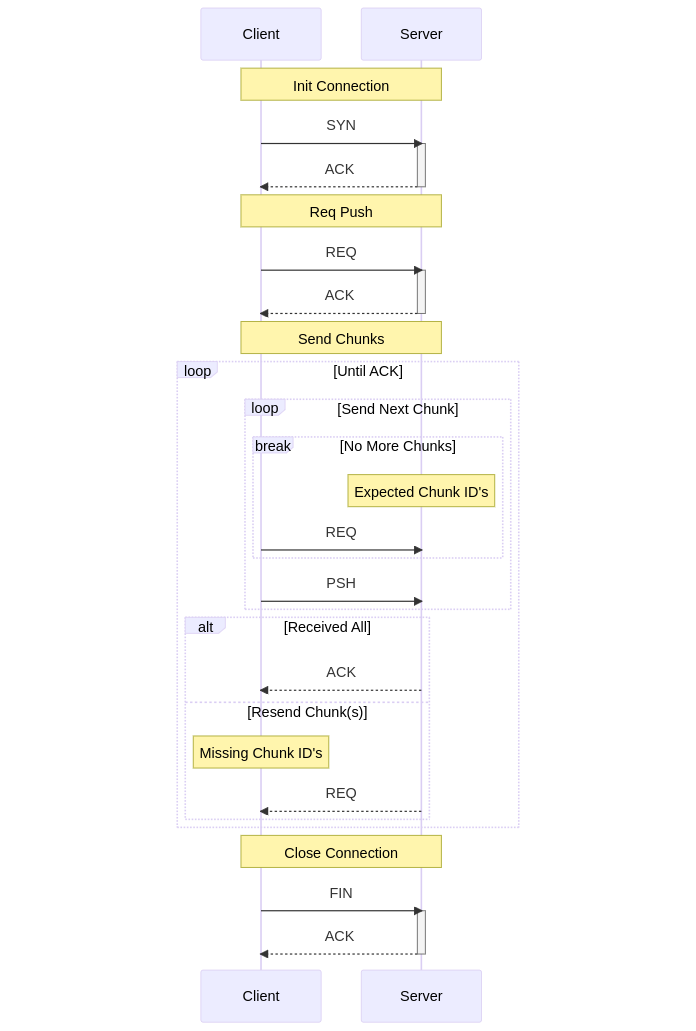
\includegraphics[width=0.8\linewidth]{p1-sequence.png}
    \caption{Prototype One Sequence Diagram}
    \label{fig:p1-sequence}
\end{figure}

\subsection*{Testing}
After the initial tests several issues in the code needed to be fixed. These are listed below (with git commit hashes):

\begin{itemize}
    \item (1e67ab) payload offset out by 1, causing payload to be incorrectly stored
    \item (dfb553) message size prediction code miss-calculates header + meta length fields, causing header and meta fields sizes to be incorrect; creating an invalid packet
    \item (35db84) client starting chunk id is 0, should be 1
    \item (455708) buffer payload was not copied (instead referenced), causing next request to alter payload values
\end{itemize}

After testing prototype one it has been found that the overhead in transferring a single file is less than the existing protocols having only "0.14\%" overhead; shown in Table~\ref{tab:prototypes-test-results}. It also sent out less packets than the existing solutions, only "39".

When testing with text files the prototype produced "7.48\%" of overhead, comparing this to the best performing existing protocol rsync which was less "5.64\%". Whilst rsync is less it is only a
"1.84\%" more, this could likely be reduced further in a future prototype.

In the next test with a collection of photos; the prototype produced a higher overhead compared to all investigated existing solutions "1.73\%", however the number of packets sent is lower "1,128". This likely points to the individual packets for transferring the physical file data having more overhead. If this was the final solution, it would be ineffective for transferring larger files since the amount of wasted data would scale with the file size.

In the last test which used a purely synthetic scenario; sending many small files sized at 1KB. The prototype produced a overhead of "~18\%" extra compared to rsync which was the best performing existing solution. Compared to the photos test, this scenario shows that this prototype has a greater amount of overhead sent for negotiating a file before transfer. However this overhead may be acceptable as rsync provides little safeguarding around file locking, compared to this prototype which if fully completed would issue an error packet before allowing a transfer to occur. Compared to the other protocols which do implement file locks (FTP and SMB2); this prototype has a smaller overhead. Looking at the number of packets sent; shows that "2,504" were sent, comparing this to rsync only "69" were sent. This is a very large difference. This prototype can only send chunks relating to the current file until the next is negotiated, whereas in rsync multiple files can be included in a single packet, making it more suitable for transferring small files, when many can fit in a single packet. Reducing the number of packets sent over the network can reduce both latency and the amount of traffic transferred allowing the bandwidth to be repurposed for another task.

This test measured a "8.0Gbps" in transfer speed. Whilst that may seem very high it is due to UDP (and the prototype) not requiring acknowledgements for each packet.

During testing it has been discovered that when many file chunks during a large transfer are lost, it will only be until the end of the transfer before they can be re-sent. This is not ideal, since on a higher latency network it could be quite a long time before the end of a transfer; resulting in a longer total transfer time. This could be improved by sending the chunks in blocks, for example 20 chunk packets could be sent then verified until either missing ones are re-sent or a new block is started. This would allow for a smaller amount of chunks to be required to be re-sent during a large transfer.

It has also been found that having two serialized fields (header, metadata) is also not ideal, since multiple complex steps have to be taken until the message can be handled. First the packet type has to be inspected, then the header must be deserialized before the metadata can be processed. This could be reduced to where only a packet type and header is sent, this would also reduce the amount of reserved space in a packet for the metadata length field; which takes up 8 bytes.

\newpage
\section{Prototype Two}
\subsection*{Solution Design}
The second prototype will focus on improving the method of sending the chunked data. This is necessary improvement, as in the event of many packets being dropped during a transfer; it will not be until the end of the transfer until the lost packets can be recovered.

To solve this without sending and waiting for acknowledgments for each packet (re-implementing TCP) a different method must be implemented. On smaller transfers the number of lost packets to recover from will be less than a larger transfer, grouping several chunks into a block of chunks then verifying each block will likely solve this issue. A sequence diagram example of a complete transfer is shown in Figure~\ref{fig:p2-sequence}.

In prototype one during the end of a transfer only three request types were sent: request to send a file, the file data and a verify packet to check if any chunks were needed to be resent. In this prototype a new request type has been added for marking the end-of-file (EOF) and ending the file transfer. The request for verification will not end the transfer; instead it is repurposed for checking for missing chunks for the current group. This will reduce the complexity of needing the server to keep a record of the blocks.

The existing protocol packet fields from prototype (headers and metadata) will stay the same. Both the client and server code will need to be altered to handle the new request type and at the client side keeping track of how many chunks are sent per block will need to be implemented. Figure~\ref{lst:p2d-offset-variables} shows the variables required for calculating blocks

\begin{lstlisting}[caption={Prototype Two Offset Variables},label=lst:p2d-offset-variables,breaklines,numbers=left,language=go]
var lastChunkID uint64 = 0
var seekOffset int = 0

chunkIDToOffset := make(map[uint64]int)

eof := false
missingChunks := make([]uint64, 0)
\end{lstlisting}


\subsection*{Testing}
After running the first test; an issue in the code discovered and had to be fixed. This is listed below (with git commit hashes):

\begin{itemize}
    \item (cae32ef) file reader cursor position not set back after a requested resend, causing incorrect data to be sent on next PSH. Fixed by seeking to stored seek offset before reading
\end{itemize}

In the first test sending a single file resulted in a higher overhead than the previous prototype, it also now has a higher overhead compared to all the tested existing solutions now showing "6.24\%". This means that implementing the transfer in blocks increased the overhead due to more packets being sent, which is shown in the results Table~\ref{tab:prototypes-test-results} going from "39" packets to "45".

In the text and photos tests prototype two still performed better than FTP and SMB2, however worse than rsync and the first prototype having "2.44\%" more overhead when transferring text and "0.19\%" more when transferring photos. This shows that the extra overhead created for handling validation of each block creates more impact on smaller files. Looking at the synthetic 1KB files test, shows the overhead to be "6.54\%" greater than prototype one. This indicates the same issue found in the text and photos test results.

In this prototype, test transfer speeds have reduced from prototype one, for example in the photos test it went from "1.9Gbps" down to "255.9Mbps", whilst slower than rsync's 1.0Gbps it reached a much greater speed than both FTP and SMB2. It likely that the extra validation added can be optimised at the software side in the last prototype.

Adding the extra message to mark a file as EOF (end-of-file), has been proved to create more overhead when sending many files. However this extra feature should allow for longer transfers to handle missing data sooner; rather than waiting until the end. The next prototype will need to ensure packet size is kept to a minimum, to reduce this overhead.

During testing an issue was discovered during transfers with multiple blocks, when they arrive out-of-order. This issue causes the chunks for different blocks to be captured incorrectly causing a corrupted file. To handle this prototype three will need to allow the receiver of a transfer to see which current chunk relates to what block. This will however increase the size of each chunk packet, but is a necessary increase in overhead for vital error checking.

Allowing the server to also know the maximum number of chunks per block could also allow memory to be pre-allocated allowing for less time to be taken allocating memory and potentially reducing the number of dropped packets during a transfer on a lower spec machine.

Due to the seen higher overhead created in both prototype one and two, the field sizes need to be reduced. Reserving 8 bytes each for the header, metadata and payload lengths causes quite a large amount of reserved space. These could be reduced from uint64 fields to uint32 reducing each field from taking 8 bytes to only 4 bytes. Also removing the metadata field as discussed in prototype one's testing would remove the need for one of the length fields.

\newpage
\section{Prototype Three}
\subsection*{Solution Design}
In prototype three which will be the last prototype, will improve on the required overhead for both the message size and required amount of processing.

Firstly the metadata field has been removed, instead opting for using the packet type field to distinguish between different packets. This will remove the need to both serialize and deserialize the two fields, shown in Table~\ref{tab:p3d-packet-fields}.

\begin{table}[h!]
    \caption{Prototype Three Packet Fields}
    \label{tab:p3d-packet-fields}
    \centering
    \begin{tabular}{ l l l }
        \hline
        \textbf{Num} & \textbf{Name}  & \textbf{Data-Type} \\
        \hline
        001          & Type           & uint8              \\
        \hline
        002          & Header Length  & uint32             \\
        \hline
        003          & Header         & protobuf           \\
        \hline
        004          & Payload Length & uint32             \\
        \hline
        005          & Payload        & binary             \\
        \hline
    \end{tabular}
\end{table}

Secondly the reserved space used for the header length and payload length has been altered. Using a reserved 8 bytes is wasteful as a packet cannot be ~18446 Petabytes in size. Instead these length fields will use uint32, which only requires 4 bytes which will allow for a header or payload to be ~4 Gigabytes in size. By not reducing any further will allow future use with IPv6 Jumbo-Frames and Jumbograms which allow for greater packet sizes to be sent. % TODO: REF

These changes will take the minimum packet size from 25 bytes to 9, which is a lot less network overhead, and allows for more file data to be sent in a single packet without loosing any functionality, shown in Listing~\ref{lst:p3d-example-structure} and Listing~\ref{lst:p3d-example-binary}.

\begin{minipage}{\textwidth}
    \begin{lstlisting}[caption={Prototype Three Example Packet Structure},label=lst:p3d-example-structure]
|-------------------|
| 1                 | <- Packet Type
| 5                 | <- Header Length
| {id: 1, mtu: 470} | <- Protobuf Header (JSON representation)
| 0                 | <- Payload Length (No Payload)
|-------------------|
\end{lstlisting}

    \begin{lstlisting}[caption={Prototype Three Example Packet Binary},label=lst:p3d-example-binary]
 1    0 0 0 5    8 1 16 214 3    0 0 0 0
 ^    ^^^^^^^    ^^^^^^^^^^^^
 |       |            |            |
Type   Header       Header       Payload
       Length                    Length
\end{lstlisting}
\end{minipage}

The next change is splitting packet types into two categories; one for requests and the other for responses. This allows the client to only need to accept responses and the sever to only accept requests, reducing the code complexity. These new packet types are shown in Table~\ref{tab:p3d-packet-types}.

\begin{table}[h!]
    \caption{Prototype Three Packet Types}
    \label{tab:p3d-packet-types}
    \centering
    \begin{tabular}{ l l l }
        \hline
        \textbf{Prefix} & \textbf{Value} & \textbf{Note}                         \\
        \hline
        REQ\_SYN        & 1              & Start connection, share capabilities  \\
        \hline
        REQ\_FIN        & 2              & Finalise connection                   \\
        \hline
        REQ\_PSH        & 10             & Request to send a file                \\
        \hline
        REQ\_PSH\_DAT   & 11             & Chunk of file data                    \\
        \hline
        REQ\_PSH\_VAL   & 12             & Request to validate current block     \\
        \hline
        REQ\_PSH\_EOF   & 13             & Mark EOF, transfer finished           \\
        \hline
        RES\_SYN        & 1              & Reply to REQ\_SYN, share capabilities \\
        \hline
        RES\_ACK        & 2              & Acknowledge REQ\_*                    \\
        \hline
        RES\_ERR\_DAT   & 10             & Chunk ID's to re-send                 \\
        \hline
    \end{tabular}
\end{table}

The last change is adding a new field to allow for requests that are related to a previous request to have a unique index. This index will allow the handling for out-of-order and old packets. This is to prevent requests such as "PSH\_VAL" and "PSH\_EOF" from triggering events multiple times, for example multiple validations may have be triggered before in prototype two due to the request ID's being the same, however the sub request ID can now be validated by the server and either handled or ignored.

\subsection*{Testing}
After running the first test several issues in the code were discovered and had to be fixed. These are listed below (with git commit hashes):

\begin{itemize}
    \item (814c3) Incomplete message sending (receive timeout method was broken)
    \item (0e422) Server unable to detect old/past messages (fixed by checking if received id is less than current)
    \item (00cee): ACK was incorrectly sent for every PSH-DAT received (fixed by removing send ack call)
    \item (eb664): ACK message did not send real request id, fixed by actually sending the request id
\end{itemize}

Testing prototype three with a single file is shown to create a greater overhead than previous prototypes, now reaching "8.99\%". Despite reducing the field sizes and removing the metadata field, it has proved ineffective, due to the added error handling required to ensure the chunk blocks are received in the correct order. However despite the increase in overhead of bytes, the number of packets sent is still smaller than the existing solutions having only exchanged "46" packets. This is likely due having a reduced amount of acknowledge requests.

In both the text and photos test the overall overhead has increased from previous prototypes, however when transferring text files it is still less than FTP and SMB2. As shown in the previous test data, this increase has likely been caused by the extra error checking.

However in the synthetic test with 1KB files, the overall overhead has decreased from the previous prototype by "\~5\%". This shows that the overhead created by field size has helped decrease the amount of unnecessary reserved space taken from each packet. The amount of packets exchanged has stayed the same still being "3,504", this is due to the extra validation being able to fit in the same number of packets because of the previously mentioned reduction in reserved space.

In this prototype, since optimising the code and removing the need for two serialization steps, the prototype is now almost the fastest in all tests. In the photos test it now is slightly faster than rsync; now reaching "1.1Gbps" in transfer speed. It is also greatly faster than rsync in the text test, performing "207.5Mbps" faster. It is also a similar transfer speed during the 1KB synthetic test, only being "1.2Mbps" slower than rsync (the fastest existing solution tested).

During testing it was also discovered that the last message sent by the client always results in multiple (as many as five) resends being sent. The cause of this issue however was not found; but does not effect the running of the prototype.

The testing of this prototype has found that when large transfers are made the overhead is greater, due to the extra error handling required because UDP has been used. This could likely be reduced in future prototypes by altering the way chunk headers are structured, for example every chunk could have a md4 hash made and each hash could be sent when a new block is started.

As discussed in a previous prototype test, when transferring many small files where an individual file does not fill an entire packet a lot of overhead is created from each file needing a separate "handshake", if rsync's methodology of bundling multiple files in one packet was used; a much lower overhead could be seen, thus allowing better utilisation of the maximum transfer speed. On a higher latency network having less packets exchanged would also decrease the amount of wait time that is needed for every acknowledgement, allowing more time to be spent transferring actual file data.

